\documentclass[12pt]{article}

\usepackage{amsmath}
\usepackage{amssymb}
\usepackage{amsfonts}
\usepackage{polski}
\usepackage{verbatim}
\usepackage[utf8]{inputenc}
\usepackage[polish]{babel}
\usepackage[T1]{fontenc}
\usepackage{graphicx}
\usepackage{caption}
\usepackage{enumitem}
\usepackage{hyperref}
\usepackage{natbib}
\usepackage{graphicx}
\usepackage{datetime}
\usepackage{multirow}
\usepackage{array}
\newdateformat{mydate}{\twodigit{\THEDAY}.\twodigit{\THEMONTH}.\THEYEAR r.}

\textheight 23.2 cm
\textwidth 6.0 in
\hoffset = -0.5 in
\voffset = -2.4 cm

\begin{document}
\begin{flushright}
	{\mydate\today}\\
\end{flushright}
\vskip10ex
\begin{center}
	\Large {\bf Analiza projektu\\}
	\small { Krzysztof Smogór \\ Piotr Widomski  }
\end{center}

\vskip15ex
\section{Streszczenie}
Celem projeku jest stworzenie systemu do zdalnej pracy opartego na architekturze rozproszonej.
System będzie umożliwiać tworzenie,
konfigurację i zarządzanie maszynami wirtualnymi. Użytkownik będzie mógł uzyskać działającą
maszynę wirtualną i pracować na niej przy pomocy protokołu zdalnego pulpitu (RDP). Maszyny
wirtualne mogą używać samego procesora lub procesora z bezpośrednim dostępem do GPU.
\section{Słownik pojęć}
\begin{itemize}
	\item Aplikacja kliencka - aplikacja uruchamiana na komputerze użytkownika, która umożliwi komunikację z systemem oraz uruchomienie zewnętrznego programu implementującego protokół RDP.
	\item Aplikacja nadzorca - aplikacja, która przetwarza zapytania od aplikacji klienckiej oraz komunikuje się z wszystkimi serwerami wirtualizacji. Na podstawie tych informacji buduje model zajętości każdego z serwerów wirtualizacji. decyduje kiedy trzeba uruchomić nowe maszyny wirtualne i na którym serwerze wirtualizacji. Dodatkowo decyduje, do której wirtualnej maszyny ma podłączyć się użytkownik proszący o utworzenie sesji.
	\item Serwer wirtualizacji - komputer, który udostępnia swoje zasoby (CPU, GPU, pamięć, przestrzeń dyskową) w postaci uruchamianych na nim maszyn wirtualnych. Dodatkowo na tym komputerze będzie uruchomiana aplikacja, która będzie odpowiadać na pytania aplikacji nadzorczej oraz wykonywać operacje na maszynach wirtualnych (uruchamianie i wyłączanie).
	\item Maszyna wirtualna CPU - jest to maszyna wirtualna, która udostępnia użytkownikowi podstawowe zasoby (procesor, pamięć i przestrzeń dyskowa) przeznaczona raczej do pracy biurowej. Uruchamiana jest na pewnym serwerze wirtualizacji z liczba zasobów zdefiniowana wcześniej w konfiguracji.
	\item Maszyna wirtualna GPU - tak jak maszyna wirtualna CPU tyle, że ma do dyspozycji przekazaną przez mechanizm GPU Passthrough kartę graficzną podłączona do serwera wirtualizacji.
	\item RDP - protokół zdalnego dostępu do pulpitu od firmy Microsoft.
	\item Sesja - jest to określenie jednorazowego dostępu do systemu przez użytkownika. Utworzenie sesji wiąże się z przypisaniem do użytkownika konkretnej maszyny wirtualnej, na której będzie pracować. Sesja kończy się w przypadku, gdy użytkownik poinformuje system o zakończeniu pracy lub gdy minie czas oczekiwania na odzyskanie połączenia po utracie połączenia.
	\item Vagrant-box\footnote{\href{https://www.vagrantup.com/docs/boxes}{Dokumentacja i opis na stronie Vagranta}} - jest to przygotowany wcześniej obraz maszyny wirtualnej, któremu można zmieniać dostępne zasoby. Uruchamiają się bardzo powtarzalnie w środowisku programu Vagrant
	\item Ansible playbook\footnote{\href{https://www.redhat.com/en/topics/automation/what-is-an-ansible-playbook#example-of-ansible-playbook}{Dokumentacja i opis na stronie Ansible'a}} - jest to pewien rodzaj skryptu konfiguracyjnego dla systemu operacyjnego, który można parametryzować i wykonywać przy starcie Vagrant-boxa.
	\item Panel administratora - jest to strona internetowa, na której administrator może sprawdzić jakie serwery wirtualizacji znajdują się w systemie oraz stan ich zasobów (wolne, zajęte oraz całkowite). 
	\item Konto użytkownika - jest to profil użytkownika w systemie, do którego ma dostęp na każdej maszynie wirtualnej. Używając przygotowanych wcześniej danych logowania może za ich pomocą logować się do maszyn wirtualnych. Będą one przechowywane w zewnętrznym (poza opisanym systemem) systemie katalogowym.
	\item Katalog użytkownika - jest to prywatny folder dostępny dla użytkownika na każdej maszynie wirtualnej. Przechowywany będzie na zewnętrznym (poza opisanym systemem) dysku sieciowym.
	\item Konfiguracja stała - jest to konfiguracja maszyny wirtualnej, która nie zmienia się w zależności od miejsca uruchomienia. Docelowo ta konfiguracja ma być zapisana w Vagrant-boxie. W potrzebie można ja także zdefiniować w odpowiednim Ansible playbooku.
	\item Konfiguracja zmienna - jest to konfiguracja wirtualnej maszyny, która zmienia się w zależności od miejsca uruchomienia. Jest definiowana w odpowiednim Ansible playbooku uruchamianym przy każdym włączeniu maszyny.
\end{itemize}

\section{Wymaganie funkcjonalne}
\subsection{Nadzorca}
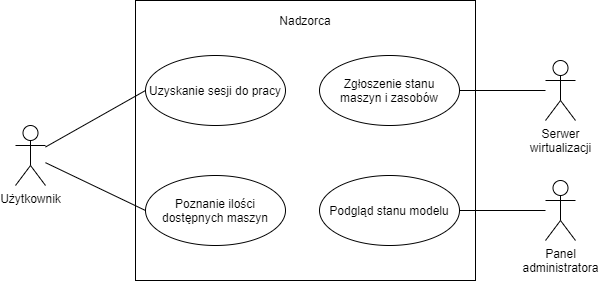
\includegraphics[width=\textwidth]{../diagrams/use_cases/overseer.png}

\begin{center}
	\begin{table}[h!]
		\begin{tabular}{|p{0.08\textwidth}|p{0.17\textwidth}|p{0.375\textwidth}|p{0.375\textwidth}|}
			\hline Aktor                                                                    & Nazwa                             & Opis                                                          & Odpowiedź systemu                                                                                                                                             \\ \hline
			\multirow{10}{=}{\rotatebox{90}{Użytkownik}}                                    & Uzyskanie sesji do pracy          & Uzyskanie sesji do pracy na maszynie wirtualnej CPU lub GPU   & Do użytkownika zostaje przydzielona maszyna wirtualna oraz zestawione połączenie RDP. W przypadku, gdy utracił on połączenie, to przydzielana jest do niego poprzednio używana maszyna, jeżeli jego sesja nie została jeszcze umorzona.                                                                     \\ \cline{2-4}
			                                                                                & Poznanie ilości dostępnych maszyn & Wyświetlanie szacowanej ilości dostępnych maszyn każdego typu & Użytkownikowi zostaje wyświetlona szacowana liczba dostępnych maszyn obliczona na podstawie informacji o dostępnych zasobach każdego z serwerów wirtualizacji \\ \hline
			\multirow[b]{5}{=}{\rotatebox{90}{\parbox{1cm}{Serwer \newline wirtualizacji}}} & Zgłoszenie dostępnych zasobów     & Serwer zgłosza nadzorcy dostępne zasoby                       & Nadzorca wykorzystuje zgłoszone zasoby do wyliczania szacowanej liczny dostępnych maszyn oraz do balansowania obciążenia serwerów wirtualizacji               \\
			\hline
		\end{tabular}
	\end{table}
\end{center}

\pagebreak

\subsection{Serwer wirtualizacji}
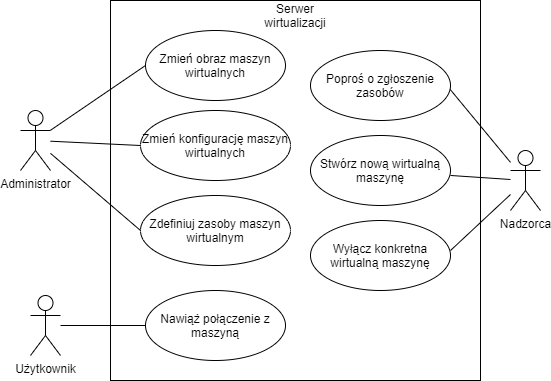
\includegraphics[width=\textwidth]{../diagrams/use_cases/virtualisation_server.png}

\begin{center}
	\begin{table}[h!]
		\begin{tabular}{|p{0.08\textwidth}|p{0.17\textwidth}|p{0.375\textwidth}|p{0.375\textwidth}|}
			\hline Aktor                                    & Nazwa                                 & Opis                                                                                                                         	& Odpowiedź systemu                                                                                                                \\ \hline
			\multirow{5}{=}{\rotatebox{90}{Użytkownik}}     & Nawiązanie połączenia z maszyną       & Użytkownik nawiązuje połączenie z maszyną wirtualną                                                                         	& Maszyna wirtualna zostaje zajęta przez użytkownika; serwer wirtualizacji rozpoczyna monitorowanie, czy sesja wciąż trwa \newline \\ \hline
			\multirow{13}{=}{\rotatebox{90}{Nadzorca}}       & Poproś o zgłoszenie zasobów           & Nadzorca wysyła do wszystkich serwerów wirtualizacji prośbę o zgłoszenie swoich używanych i wolnych zasobów                  	& Serwer wirtualizacji informuje nadzorcę o stanie swoich zasobów                                                                  \\ \cline{2-4}
															& Stwórz nową wirtualna maszynę         & Nadzorca prosi serwer wirtualizacji o stworzenie nowej wirtualnej maszyny dla danego użytkownika na wybranym typie maszyny                											& Serwer wirtualizacji tworzy wirtualna maszynę i udostępnia możliwość połączenia się z nią                                                    \\ \cline{2-4}
															& Wyłącz konkretna wirtualna maszynę    & Nadzorca prosi serwer wirtualizacji aby wyłączył konkretna wirtualna maszynę.                											& Serwer wirtualizacji wyłącza konkretna wirtualna maszynę oraz pilnuje aby na pewno się wyłączyła.                                                    \\ \hline
			\multirow{11}{=}{\rotatebox{90}{Administrator}} & Zmień obraz maszyn wirtualnych        & Zmiana obrazu źródłowego maszyn wirtualnych                                                                                  	& Zdefiniowany przez administratora vagrant-box jest używany przez serwery wirtualizacji                                           \\ \cline{2-4}
			                                                & Zmień konfigurację maszyn wirtualnych & Zmiana zmiennej konfiguracji maszyn wirtualnych                                                                              	& Zmodyfikowany ansible playbook jest używany przez serwery wirtualizacji                                                          \\ \cline{2-4}
			                                                & Zdefiniuj zasoby maszyn wirtualnych   & Zmiana ilości zasobów przydzielanych na każdy z typów maszyn wirtualnych oraz łączną ilość zasobów przeznaczonych na maszyny 	& Zmodyfikowana konfiguracja zasobów będzie wykorzystowana przez serwer wirtualizacji przy kolejnym uruchomieniu                   \\
			\hline
		\end{tabular}
	\end{table}
\end{center}

\pagebreak

\subsection{Panel administratora}
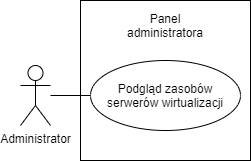
\includegraphics[width=\textwidth]{../diagrams/use_cases/admin_panel.png}

\begin{center}
	\begin{table}[h!]
		\begin{tabular}{|p{0.08\textwidth}|p{0.17\textwidth}|p{0.375\textwidth}|p{0.375\textwidth}|}
			\hline Aktor                                                                    & Nazwa                                  & Opis                                                              & Odpowiedź systemu                                                                                                                                                    \\ \hline
			\multirow{7}{=}{\rotatebox{90}{Administrator}}                                  & Podgląd zasobów serwerów wirtualizacji & Wyświetlanie wolnych oraz zajętych zasobów serwerów wirtualizacji & Wyświetlenie zasobów poszczególnych serwerów wirtualizacji, liczby zajętych maszyn oraz szacowanej liczby wolnych maszyn \newline\newline                            \\ \hline
			\multirow[b]{6}{=}{\rotatebox{90}{\parbox{1cm}{Serwer \newline wirtualizacji}}} & Zgłoszenie dostępnych zasobów          & Serwer zgłosza panelowi administratora dostępne zasoby            & Panel administratora wykorzystuje zgłoszone zasoby do wyliczania szacowanej liczny dostępnych maszyn oraz wyświetlania zasobów poszczególnych serwerów wirtualizacji \\
			\hline
		\end{tabular}
	\end{table}
\end{center}

\newpage
\section{Wymaganie niefunkcjonalne}

\begin{center}
	\begin{table}[h!]
		\begin{tabular}{|p{0.2\textwidth}|p{0.2\textwidth}|p{0.6\textwidth}|}
			\hline Grupa wymagań                            & Nr wymagania & Opis                                                                                                                                                                    \\ \hline
			\multirow[t]{8}{=}{Użytkowanie (Usability)}     & 1            & Aplikacja kliencka ma działać na systemach operacyjnych GNU/Linux oraz MS Windows                                                                                       \\ \cline{2-3}
			                                                & 2            & Aplikacja kliencka musi udostępniać możliwość użycia własnego klienta RPD do nawiązania połączenia z maszyną wirtualną                                                  \\ \cline{2-3}
			                                                & 3            & Maszyny wirtualne muszą mieć dostęp do systemu przechowującego konta użytkowników wraz z ich katalogami domowymi                                                        \\ \hline
			\multirow[t]{7}{=}{Niezawodność (Reliability)}  & 4            & System musi być odporny na awarie poszczególnych serwerów wirtualizacji i kontynuować działanie w sposób niezauważalny dla użytkowników nie używających danego serwera. \\ \cline{2-3}
			                                                & 5            & Awaria nadzorcy może spowodować uniemożliwienie rozpoczęcia nowych sesji, ale nie może przerwać istniejących sesji                                                      \\ \hline
			\multirow[t]{10}{=}{Wydajność (Performance)}    & 6            & Łącznie zużywane zasoby przez maszyny wirtualne na poszczególnym serwerze wirtualizacji nie mogą przekroczyć wcześniej zdefiniowanych limitów                           \\ \cline{2-3}
			                                                & 7            & Nadzorca musi balansować obciążenie serwerów wirtualizacji                                                                                                              \\ \cline{2-3}
			                                                & 8            & W systemie zawsze musi istnieć jedna działająca maszyna wirtualna nie połączona z żadną sesją, aby można było ją szybko przydzielić użytkownikowi                       \\ \cline{2-3}
			                                                & 9            & Zwolnione maszyny wirtualne, które nie są wykorzystywane jako zapas, muszą być wyłączane                                                                                \\ \hline
			\multirow[t]{3}{=}{Utrzymanie (Supportability)} & 10           & Możliwe jest działanie więcej niż jednego nadzorcy w systemie, w celu zwiększenie dostępności lub przeprowadzenia prac utrzymaniowych                                   \\
			\hline
		\end{tabular}
	\end{table}
\end{center}

\section{Analiza ryzyka}

\begin{tabular}{| c | c |}
	
\end{tabular}
\section{Harmonogram projektu}
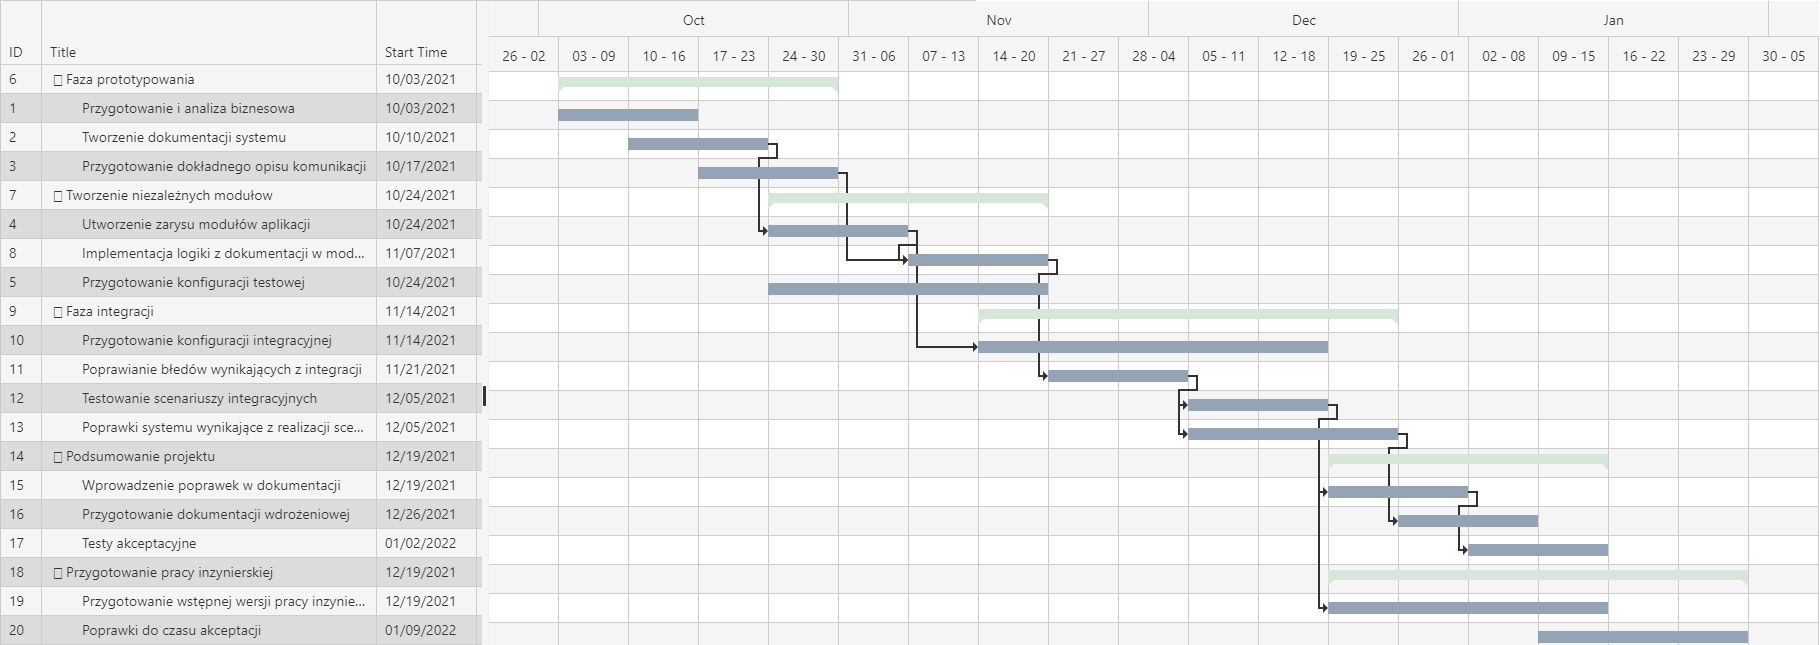
\includegraphics[width=\textwidth]{resources/harmonogram.png}

\end{document}